\documentclass[Main]{subfiles}
\begin{document}

\chapter{}
This chapter will cover the fundamentals in data distribution service (DDS), explaining the concept of middleware and DDS for real-time systems.
\\
\section{Middleware}
In distributed systems, where multiple independent computers are connected on a network due to collaborating in achieving the same goal. These computers can be placed with different geographical locations and have different operating systems (OS) \cite[p. 2]{Tanenbaum}.
\\ To make the development of a distributed system easier developers can use middleware, which is software between the application and the physical layers on the computer. The middleware contributes to the development as it hides the problems that can occur due to different software, hardware and OS's from each application \cite[p. 3]{Tanenbaum}.

\begin{figure}[H]
\centering
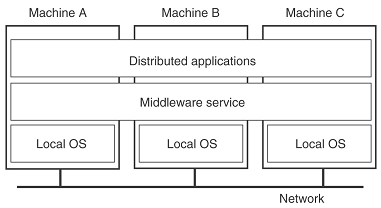
\includegraphics[scale=1]{Figure/Middleware.png}
\caption{A distributed system with middleware \cite[p. 3]{Tanenbaum}}
\label{Fig:Middleware}
\end{figure}

Each application is offered the same interface through the middleware layer which extends over multiple machines \cite[p. 3]{Tanenbaum}. The middleware is a principle that makes it easier for developers to scale a distributed system, as the developer can focus on the interface to the middleware and not the layers beneath. This makes the environment homogeneous as the differences in network technology, hardware architecture, OS, programming languages and geographical locations etc. is not to be taken care of by developers \cite{DDS-slides} \cite[p. 68]{Coulouris}.
\\
To support the different programming languages used in the applications the middleware supports the Interface Definition Language (IDL). It is a standard language for defining the interfaces which enables communication between applications that do not share programming language. This means that each application transform the programming langauge into IDL and transfer it into the middleware \cite{DDS-slides} \cite{RTI} \cite{wiki-idl}.
\\
Middleware is useful when developing large and complex distributed systems as it connects the different parts with a "pipe" that makes data-sharing and communication efficient \cite{DDS-slides} \cite[p. 68]{Coulouris}. It should be considered that the middleware-software should be installed on all the involved computers which can raise the CPU load. Depending on the type of hardware that is used the developers should choose a sufficient middleware \cite{DDS-slides}.
\\
\\
When choosing between middlewares it is important to know which standard the different middlewares are using. There is a lot of standards that the middleware can support, e.g. which network the middleware supports or if the middleware supports a medical standard for transferring images and data between devices in the medical industry \cite{DDS_slides}.\\
There are various implementations of the standards e.g. OpenDDS by Object Computing Inc. which is an open source implementation. Among the commercial implementations Real-Time Innovations (RTI) has developed a middleware called Connext.

Mia - Skal der skrives mere her? Synes Christian sagde noget men har pt glemt det - ved ikke om du går lidt i dybden med det i dit afsnit? Det var noget de forskelilge standarder, mens synes vi går i dybden med det når vi forklare DDS.
Lasse - nej, jeg synes det er fint som det står :)
\\\\
A concrete implementation of this middleware in a distributed system is seen below.
\begin{figure}[H]
\centering
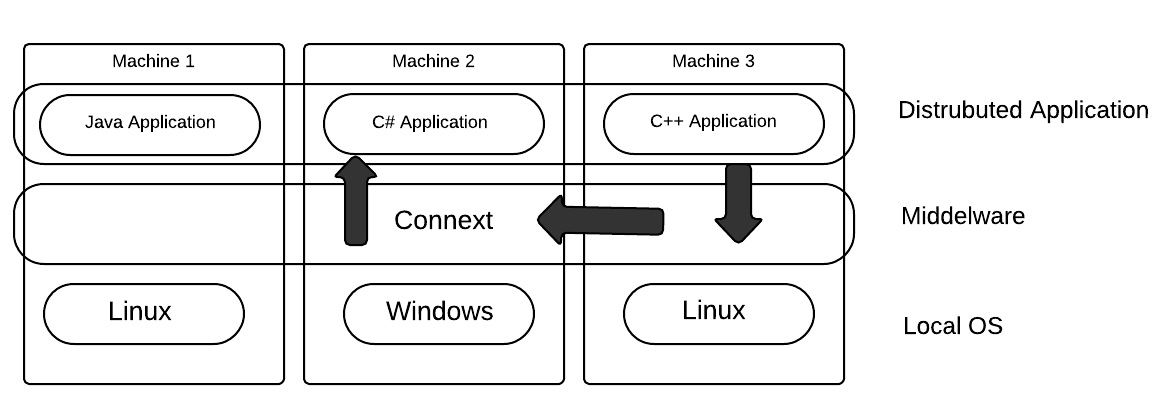
\includegraphics[scale=0.4]{Figure/MiddelwareImplementation.png}
\caption{Connext in a distributed system}
\end{figure}

The figure shows, that a C++ application on Machine 3 is transferring data to the middleware. The middleware then handle and transform it, so it can be used on Machine 2, even if the programming languages and the machines are different from each other. 
\\
The communication in the middleware is performed by a publish-subscriber paradigm, called Data-Centric publish-subscribe, which is explained in details in the next section. Other forms of middelware communication paradigms is e.g. Message Passing, Message queuing, Remote procedure call and derivatives and etc.\cite{DDS-slides}.\\
These communication paradigms in middleware decouples data producers and consumers in different ways and can be categorized into three different decouplings; space, time and flow decoupling. \\
Space decoupling is if the producers and the consumers do not know each other, which means that they do not have a reference to each other and do not know the location of each other.
\\
Time decoupling is if the interaction is asynchronous which means that the data being passed can be used later and not when it is received. An example on an asynchronous communication could be a mail client which receives mails, but the mails can be read at a later time than when it arrived. A synchronous communication could be a phone call where it is only possible to talk if the recipient is answering the call. \\
Flow decoupling is if the data production and consumption are not blocking the flow for the producer or the consumer. This means that the producer and the consumer do not block each other when they use the data being passed between them. 

\section{Data distribution service for real-time systems}
The DDS is a specification standard, approved by the Object Management Group (OMG), that facilitates data-communication through the data-centric publish/subscribe paradigm \cite{RTI}. The DDS standard supports deterministic data-delivery (if the underlying data-link and physical layer supports it), a large number of configuration parameters and a low overhead on memory and CPU \cite{DDS-slides}.\\
The specification for DDS consists of two distinct sections; Data Logical Reconstruction Layer (DLRL) and Data-Centric Publish-Subscribe (DCPS) \cite{DDS-slides}.


\begin{figure}[H]
\centering
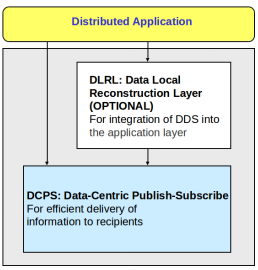
\includegraphics[scale=0.8]{Figure/DLRLandDCPS.png}
\caption{The two sections in the DDS specification \cite{DDS-slides}}
\label{Fig:DLRL}
\end{figure}

The DLRL is an optional upper layer that allows a simpler integration of the DDS into the application layer. It provide a more natural access to data as it updates a local copy of the data, which allows the application to access the data as if local \cite{DDS-slides}. It outlines how an application can interface with DCPS data fields. According to Gerardo Pardo from RTI no DDS vendors supports the DLRL any more \cite{DLRL-support}.\\
The DCPS is the lower layer which the application uses to communicate with other DDS-enabled applications; it provides efficient delivery of the proper information to the proper recipients \cite{wiki-DDS}. The DCPS comprises the following entities:

\begin{figure}[H]
\centering
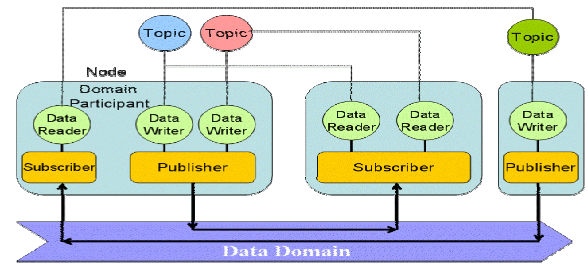
\includegraphics[scale=0.8]{Figure/DDSentities.png}
\caption{The DDS/DCPS entities \cite{RTI}}
\label{Fig:Entities}
\end{figure}

\begin{itemize}
  \item \textbf{Domain}\\The basic construct that binds the individual applications together and where data is send and received from. The domain is the defined communication-area in which the data is being shared.
  \item \textbf{Domain participant}\\This object enables the developer to specify default Quality of Service (QoS) parameters for all entities in the corresponding domain.
  \item \textbf{Data Writer}\\The primary access point for an application to publish data into the data domain. The Data Writer is configured with the wanted QoS-settings which enables it to write data of a particular type. All data that is going to be transferred is written by the Data Writer with a simple write-method. When the write is executed the data will be passed to the publisher. 
  \item \textbf{Publisher}\\The publisher is a container to group individual Data Writers; it can have many Data Writers. The publisher can also be configured with QoS-parameters and can apply these parameters to all the Data Writers it contains.
  \item \textbf{Data Reader}\\The Data Reader is the primary point to access data that has been received by a Subscriber. The Data Reader can read data from Data Writers if the data has the same type; the reader has a single Topic.
  \item \textbf{Subscriber}\\As for the Publisher the Subscriber is a container that groups the Data Readers; it can have many Data Reader. When data is available the Subscriber can notify the application in one of three ways:
  \begin{itemize}
  \item Listener Callback Routine which makes DDS run our own specific software to access data as soon as it arrives.
  \item Polling the Data Reader to check if data is available.
  \item Conditions and WaitSets where the application access the data from the Data Reader when specified conditions is met.
  \end{itemize}
  \item \textbf{Topic}
  \\\cite{RTI} \cite{opendds}
\end{itemize}

The figure below shows another conceptual view on publication, subscription and topic: 

\begin{figure}[H]
\centering
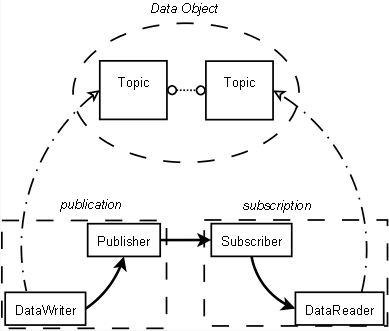
\includegraphics[scale=0.7]{Figure/PublicationAndSubscription.png}
\caption{A simple conceptual view of publication and subscription \cite{ddsopen}}
\end{figure}




As described in the section above the RTI Connext implements the DDS standard


\end{document} 